\chapter{Avaliação Experimental}
\label{avaliacao}

\section{Metodologia}
\label{sec:metodologia}

%\begin{itemize}
%\item o que e como avaliar
%\item quais programas serão utilizados na avaliação
%\end{itemize}

% Reordenar frases: A segunda passa a ser a última.
Para avaliar o desempenho do compilador JIT desenvolvido, foi feita uma
análise detalhada com seis \textit{benchmarks} simples. Todos os
testes foram realizados em um computador com processador Intel Core 2
Duo, modelo E4700; memória principal de 2 GiB de 666 MHz, DDR2 DIMM;
\textit{kernel} Linux 2.6.32-25-generic. Foram coletados dados macro acerca
de: tempo total de execução (\textit{wallclock}),
tempo da compilação JIT, tempo exclusivo de execução de procedimentos
com e sem o JIT desenvolvido. Também coletou-se dados detalhados
envolvendo a arquitetura do processador utilizado.
% XXX Talvez coletar mais usando o PAPI, cache l1 hit/miss
Em todos os casos fez-se uso da ferramenta PAPI \cite{papisite}
 4.1.1 e,
com exceção do \textit{wallclock}, a implementação da \texttt{Tcl} foi
instrumentada para coletar os dados específicos. Foram utilizadas duas
versões da \texttt{Tcl} 8.5.7, a padrão e outra modificada que inclui
o compilador JIT, ambas compiladas com gcc \verb!-O2!.


\section{Benchmarks}

A implementação atual do compilador cobre apenas um subconjunto
da linguagem \texttt{Tcl}, portanto alguns \textit{benchmarks}
específicos e rudimentares foram criados para possibilitar
uma avaliação inicial. Há uma suíte de testes para a \texttt{Tcl}, a Tclbench
\cite{tclbench-site}, porém somente uma quantidade bastante pequena dos
testes lá existentes podem ser executados com sucesso neste sistema e,
portanto, seu uso não foi considerado.

Em todos os \textit{benchmarks} faz-se uso de um parâmetro $n$ com
significado específico para cada teste. Os \textit{benchmarks}
utilizados foram:
% (códigos ver apêndice
%\ref{apendice-bench}).

\begin{description}
\item[fact] Fatorial iterativo. Calcula $n$ vezes o fatorial dos
  números de 1 a 12
\item[gcd] Máximo divisor comum. Este teste é realizado
  para todos os elementos do produto cartesiano
 $I \times J = \{(i, j) \mid i \in \mathbb{N} \wedge j \in \mathbb{N},
 i \le n \wedge j \le n\}$
\item[gray] Calcula o código gray \cite{graycode} de um número;
  quase um \textit{microbenchmark}. O parâmetro $n$ indica um
  intervalo $[0, n)$ para ter seus respectivos códigos gray gerados.
\item[prime] Verifica se um número é primo ou não. Parâmetro $n$
  define o intervalo ($[0, n]$) de números a serem verificados.
\item[sum$_1$] Somatório de números naturais no intervalo
 $[1, i]$, onde $i$ representa o número da iteração atual no intervalo
 $[1, n]$
\item[sum$_2$] Somatório definido por:
\[ \sum_{i=0}^k a_i\mbox{, onde } a_i = \left\{
    \begin{array}{c l}
      i & \mbox{se } i \mbox{ mod } 4 = 0 \\
      -i & \mbox{se } i \mbox{ mod } 3 = 0 \\
      0
    \end{array}
  \right.
\] com $k$ equivalente a iteração atual no intervalo $[1, n]$
\end{description}


\section{Desempenho}

Para verificar o desempenho a nível macro do compilador JIT,
realizou-se primeiramente a coleta do tempo gasto em execuções
completas. As Figuras
\ref{fig:fact-tempo}, \ref{fig:gcd-tempo}, \ref{fig:gray-tempo},
\ref{fig:prime-tempo}, \ref{fig:sum1-tempo} e \ref{fig:sum2-tempo}
apresentam os dados obtidos para os seis \textit{benchmarks}
distintos. Em todos os casos foram realizadas 100 execuções com tamanho de
$n$ uniformemente espaçado entre os valores mínimo e máximo utilizados.

\begin{figure}[ht!]
  \centering
  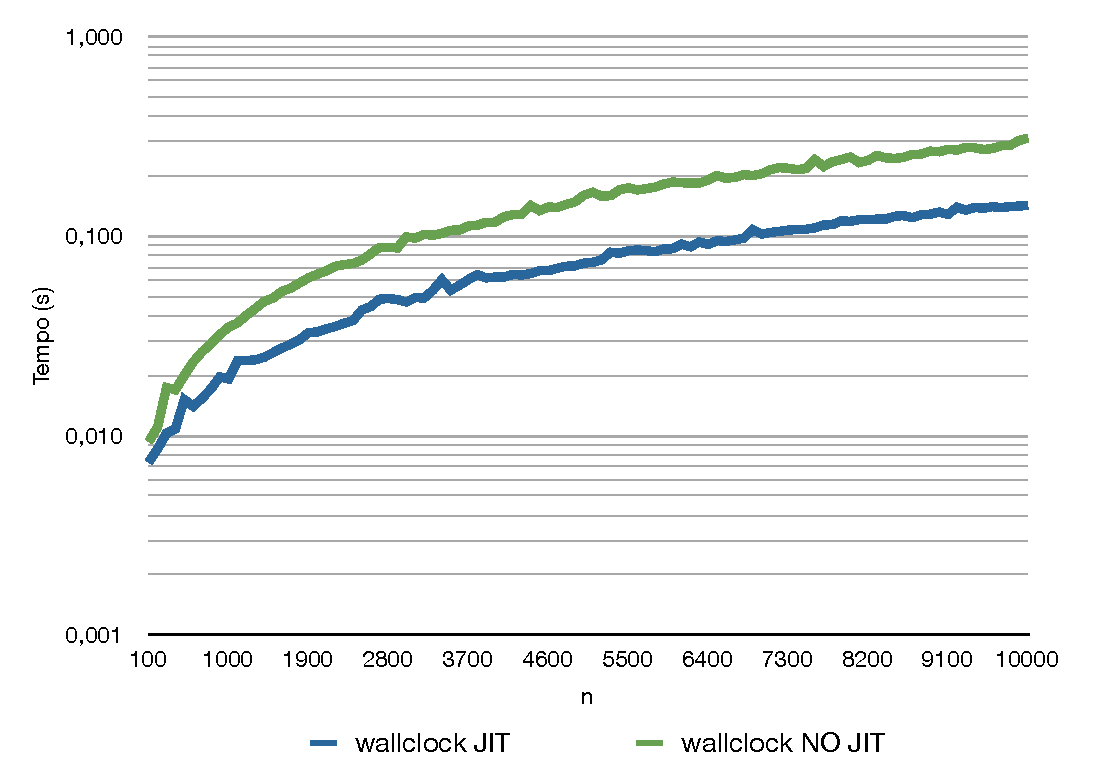
\includegraphics[scale=0.70]{figs/fact_tempo}
  \caption{Tempo total de execução para fact \label{fig:fact-tempo}}
\end{figure}
\begin{figure}[ht!]
  \centering
  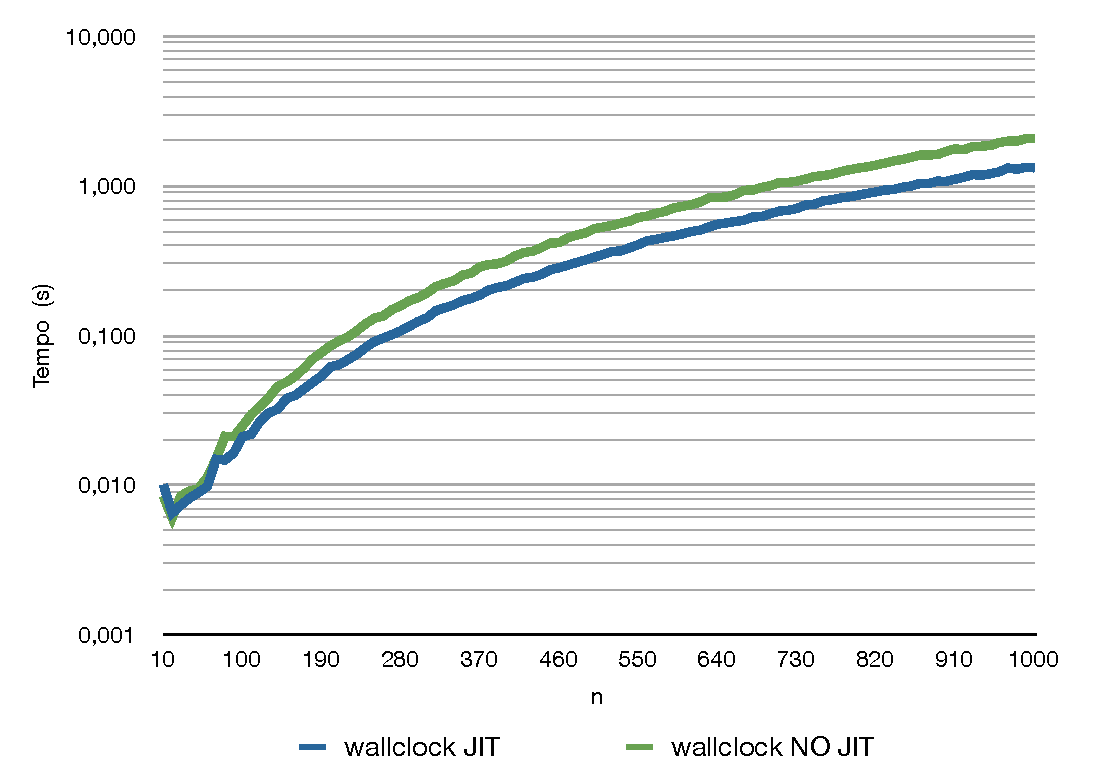
\includegraphics[scale=0.70]{figs/gcd_tempo}
  \caption{Tempo total de execução para gcd \label{fig:gcd-tempo}}
\end{figure}
\begin{figure}[ht!]
  \centering
  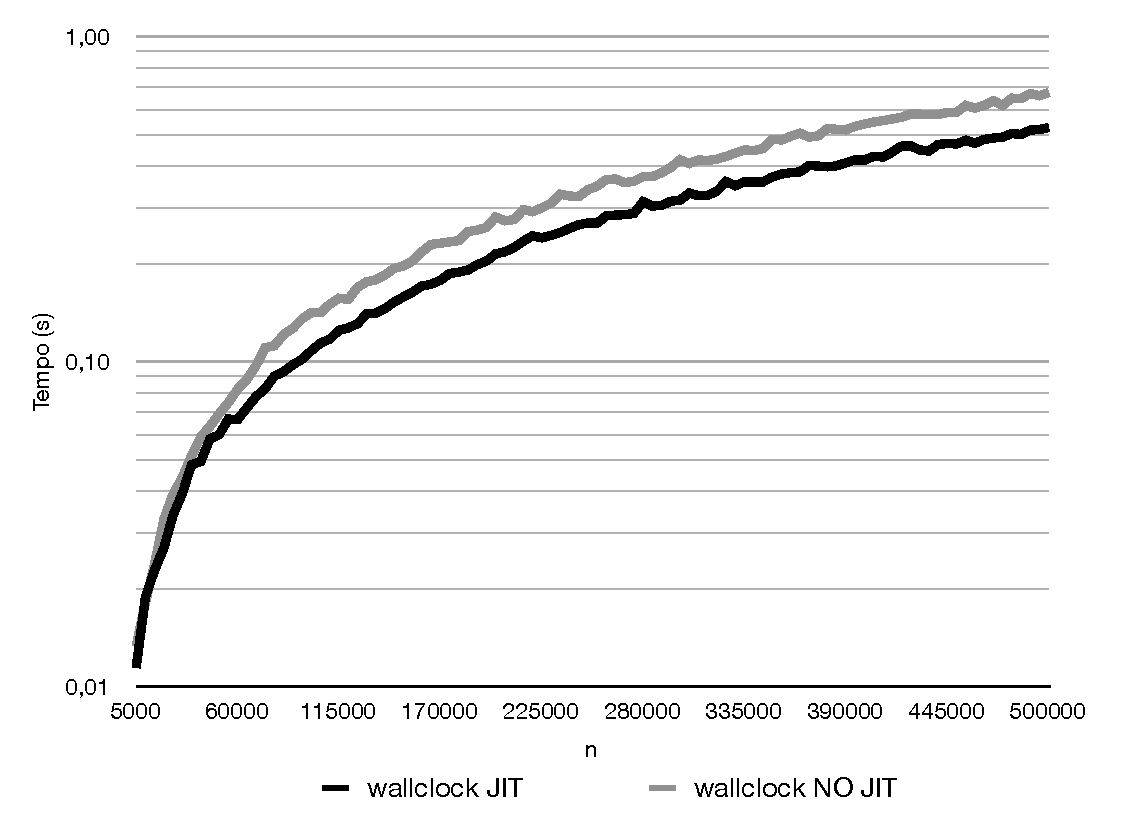
\includegraphics[scale=0.70]{figs/gray_tempo}
  \caption{Tempo total de execução para gray \label{fig:gray-tempo}}
\end{figure}
\begin{figure}[ht!]
  \centering
  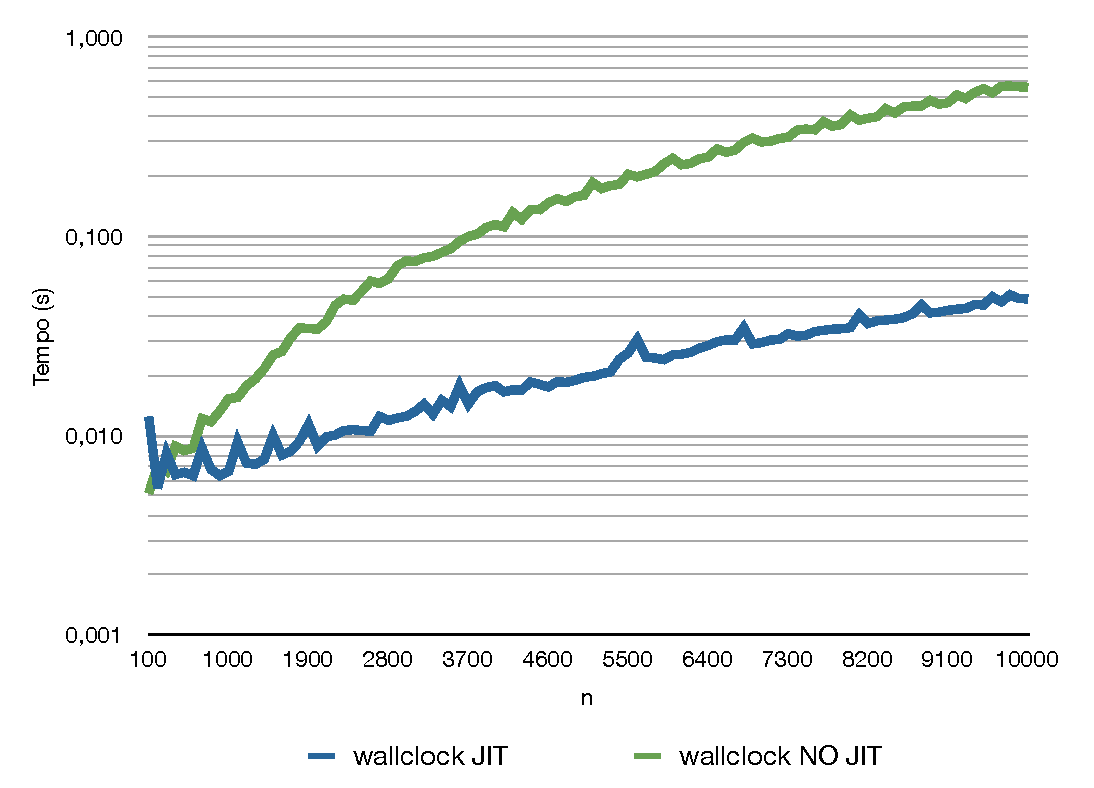
\includegraphics[scale=0.70]{figs/prime_tempo}
  \caption{Tempo total de execução para prime \label{fig:prime-tempo}}
\end{figure}
\begin{figure}[ht!]
  \centering
  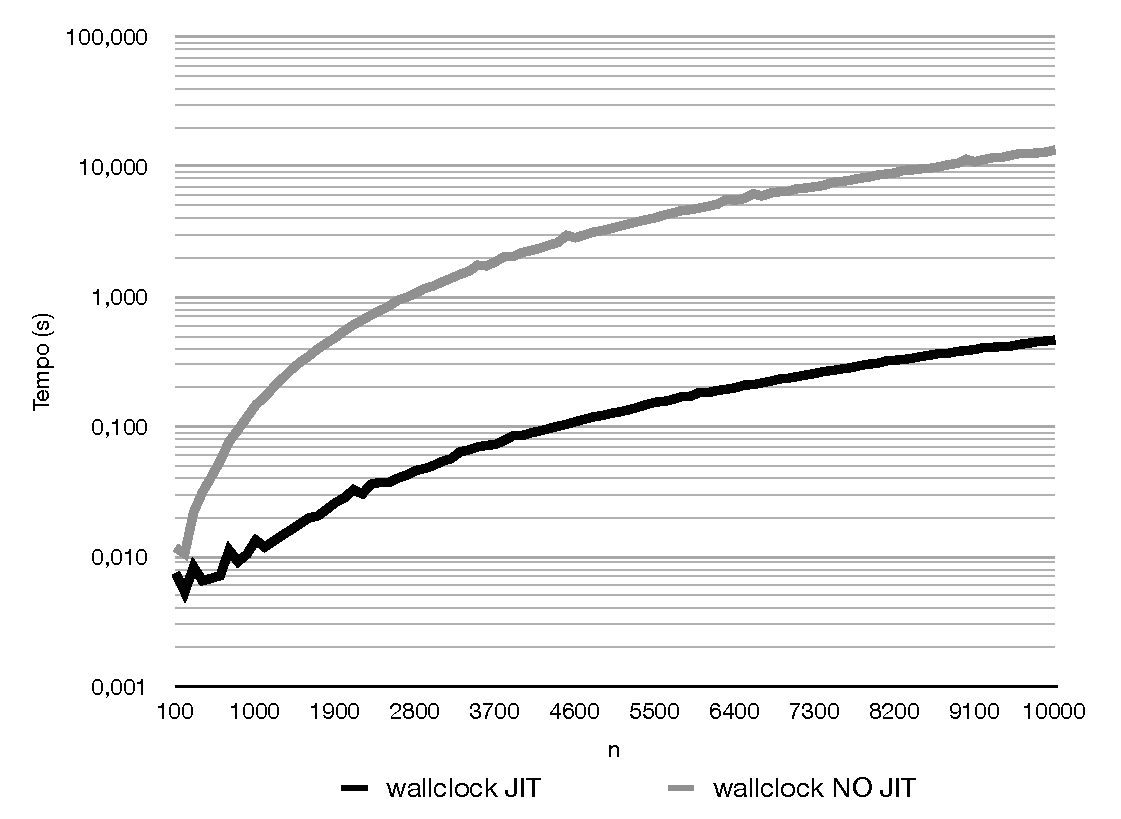
\includegraphics[scale=0.70]{figs/sum1_tempo}
  \caption{Tempo total de execução para sum$_1$ \label{fig:sum1-tempo}}
\end{figure}
\begin{figure}[ht!]
  \centering
  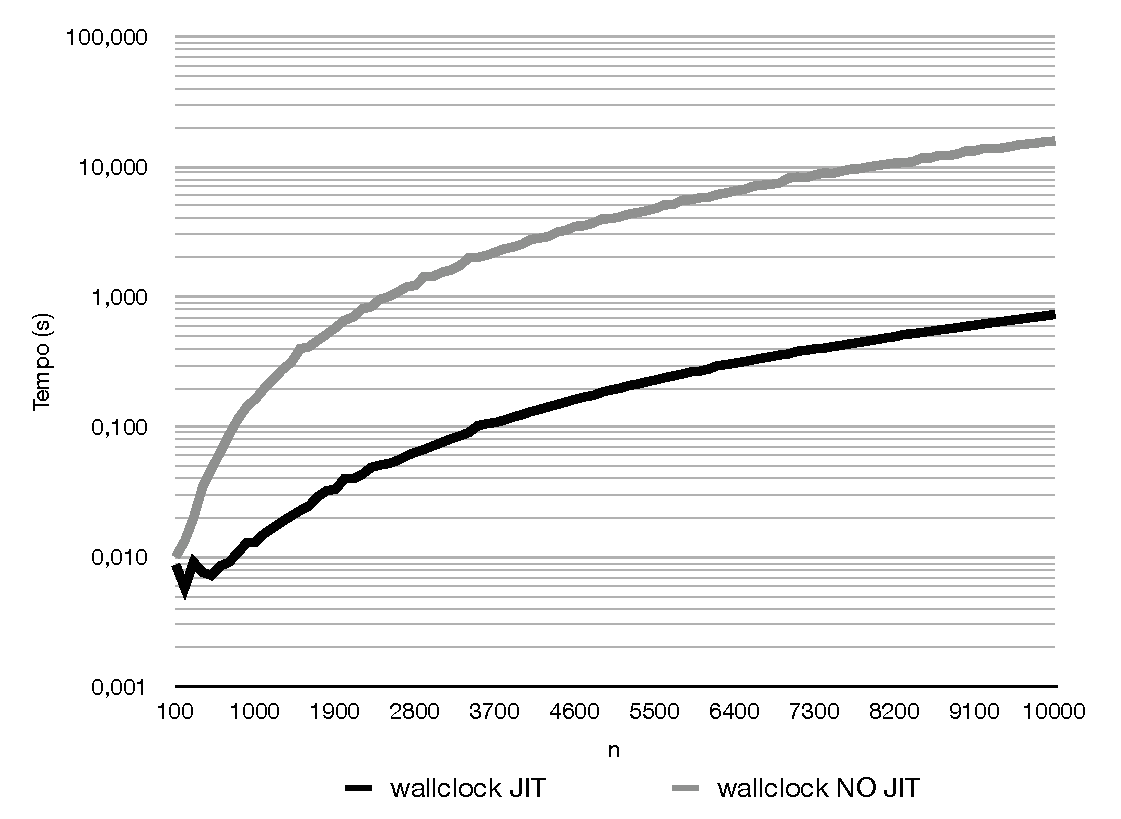
\includegraphics[scale=0.70]{figs/sum2_tempo}
  \caption{Tempo total de execução para sum$_2$ \label{fig:sum2-tempo}}
\end{figure}

Em grande parte das execuções, a linha que indica o tempo com uso
do compilador JIT permaneceu abaixo da linha do interpretador padrão da
\texttt{Tcl}. Isto era esperado em vista das restrições do sistema
implementado.

Dentre os testes, \textbf{sum$_1$} (Figura
\ref{fig:sum1-tempo}) apresenta a maior
redução (mais de 20 vezes em média). Isto é reflexo do código ali
contido, sendo constituído principalmente de deslocamentos entre
endereços da pilha e soma de inteiros. O gerador de código atual
consegue eliminar boa parde de toda a movimentação de objetos de tipo
\verb!Tcl_Obj!, realizando todas as conversões de \verb!Tcl_Obj! para
inteiro (se possível) num bloco básico especial dedicado para esta
tarefa.
% XXX esse bloco básico especial é aquele gerado na reordenação
% de instruções
Com isso, é possível trabalhar com instruções de máquina que operam
diretamente sobre esses valores inteiros e elimina-se muito do
\textit{overhead} existente na máquina virtual \texttt{Tcl}. O teste
\textbf{sum$_2$} (Figura \ref{fig:sum2-tempo}) também
apresentou um ganho significativo, apesar de fazer uso de divisão por
constante com uso da \verb!IDIV!. Esta é a forma mais simples e geral de
realizar a divisão, mas os compiladores otimizadores a evitam
\cite{opt-invariantintdiv} por consumir muitos ciclos.
%XXX Será que ficou claro por que teve os ganhos ?

Os \textit{benchmarks} \textbf{fact} (Figura \ref{fig:fact-tempo}),
\textbf{gcd} (Figura \ref{fig:gcd-tempo}) e \textbf{gray} (Figura
\ref{fig:gray-tempo}) não apresentam resultados tão expressivos. No
caso do \textbf{gray}, tem-se que ele é o teste que requer a menor
quantidade de \textit{bytes} para sua codificação e talvez
procedimentos muito pequenos não sejam altamente beneficiados pelo
compilador atual. Os outros dois têm tamanho próximo do
\textbf{sum$_1$}, mas fazem uso de instruções de multiplicação ou
divisão.

Nota-se que \textbf{prime} (Figura \ref{fig:prime-tempo}),
e \textbf{sum$_2$} apresentaram um comportamento
diferenciado nas primeiras execuções. Apesar de $n$ aumentar,
houve um decréscimo de tempo entre a primeira e a segunda
execução nestes casos ao passo em que isto não ocorre quando o código é
interpretado.
Coincidentemente \textbf{prime} e \textbf{sum$_2$} são os que
mais requerem do compilador dinâmico, sendo necessário emitir, na
etapa final, 725 e 609
\textit{bytes}, respectivamente, e, portanto, requerem um tempo maior
na compilação antes da primeira execução nativa. Entretanto, deve-se
notar que os tempos de execução em questão são baixos e que pequenas
modificações no ambiente do sistema operacional podem causar pequenas
flutuações e anomalias nos resultados. Com estes dados, ainda não é
possível concluir que, de fato, o tempo de compilação influenciou
nesse fenômeno observado.

%XXX Quantidade de execuções, nao influencia as curvas ? Talvez
%compilar algo depois de 1 execução nao tenha muita vantagem.

%prime: 768 bytes
%sum2: 633 bytes
%gcd: 401 bytes
%sum1: 363 bytes

%fact: 367 bytes
%gray: 179 bytes

Para facilitar a visualização da diferença de desempenho,
destaca-se a Figura \ref{fig:media-tempo}. O \textit{microbenchmark}
apresenta o menor ganho (cerca de 25\%) mas pode-se verificar que o
tempo gasto pelo laço que
executa o teste domina o tempo total. Somente para executar
\verb!for {set i 0} {$i < $n} {incr i} { .. }!, no maior
teste, gasta-se cerca
de 0,45 segundos, deixando menos de 0,07 segundos para efetivamente
executar o \verb!gray!.

\begin{figure}[ht]
  \centering
  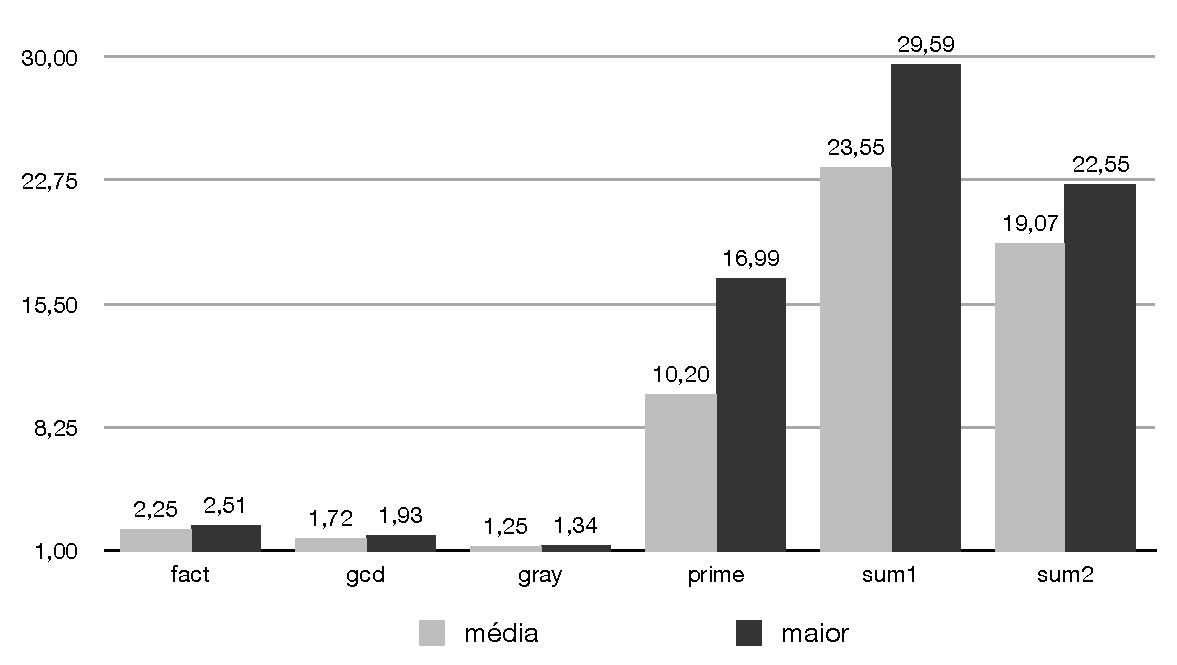
\includegraphics[scale=0.70]{figs/melhoria}
  \caption{Melhoria em relação ao tempo do interpretador padrão (vezes) \label{fig:media-tempo}}
\end{figure}

Apesar de apresentar resultados positivos, os dados exibidos até
agora estão ``contaminados'' com \textit{overhead} herdado da
máquina virtual \texttt{Tcl}. Para determinar quanto tempo exatamente
é consumido pelo compilador dinâmico, mais dois testes foram
realizados.

Com a Figura \ref{fig:tempo-compilacao} verifica-se que o tempo de
compilação tem influência quase nula no tempo total, custando entre
$49 \times 10^{-6}$ e $79 \times 10^{-6}$ segundos. Também nota-se que
o crescimento do tempo de compilação não acompanha o crescimento dos
\textit{bytes} na mesma proporção.
A linha de tendência 1, para os \textit{bytes}, é
descrita por $y = 10,143x^2 + 31,771x + 168.8$ e apresenta um índice
de correlação com os dados de 0,9379. Enquanto isso, a linha de
tendência 2 é dada por $y = 1,3571x^2 - 3,9x + 52,4$ com índice de
correlação de 0,9876. Onde $1 \le x \le 6$. A tendência é que o tempo
de compilação continue baixo.

\begin{figure}[ht]
  \centering
  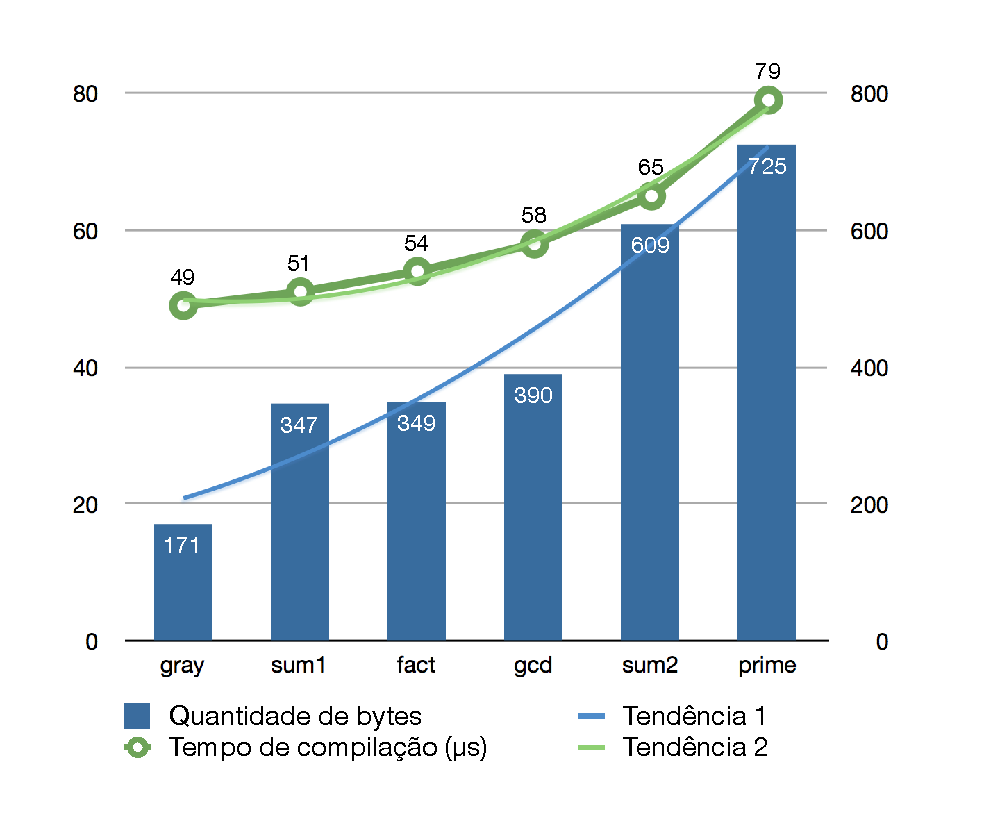
\includegraphics[scale=0.71]{figs/tempo_compilacao}
  \caption{Quantidade de bytes x86 e tempo de compilação \label{fig:tempo-compilacao}}
\end{figure}

A Tabela \ref{tabela-execacc} apresenta os resultados do último teste
desta seção. Para chegar-se a estes dados, utilizou-se dados dos
resultados anteriores para $n$ no maior caso e depois $n$ foi fixado
de acordo com o valor máximo utilizado nos testes específicos de
\textit{wallclock} e, então, foram feitas 10 execuções em cada
situação nova e tomada a média do tempo.

\begin{table}[ht!]
  \caption{Tempo de execução dos \textit{benchmarks} no maior caso\label{tabela-execacc}}
  \centering
  \begin{tabular}{l c c c c c c r}
    \toprule
& \multicolumn{2}{c}{JIT (s)} & \multicolumn{2}{c}{NO JIT (s)} \\
\cmidrule(r){2-3} \cmidrule(r){4-5}
    \textit{Benchmark}  & Total & Exclusivo & Total & Exclusivo & Melhoria (vezes) \\
    \midrule
    fact & 0,14 & 0,04  & 0,30 & 0,19  & 4,75    \\
    gcd & 1,32 & 0,37  & 2,08 & 1,14  & 3,08   \\
    gray & 0,52 & 0,13  & 0,57 & 0,17   & 1,30   \\
    prime & 0,04 & 0,03 & 0,56 & 0,54   & 18,00     \\
    sum$_1$ & 0,46 & 0,44 & 10,60 & 10,22   & 23,22    \\
    sum$_2$ & 0,73 & 0,71 & 11,61 & 10,87   & 15,30     \\
    \bottomrule
  \end{tabular}
\end{table}

% XXX Coletar novamente tempo para prime, sum1 e sum2 nos testes acima.
%XXX Comentar Tabela \ref{tabela-execacc}
A última coluna da Tabela \ref{tabela-execacc} refere-se a melhoria na
nova situação: tempo exclusivo com JIT e sem JIT. Os
\textit{benchmarks} \textbf{fact}, \textbf{gcd} e \textbf{gray} que
tinham tido o menor ganho (Figura \ref{fig:media-tempo}) melhoraram um
pouco se comparados somente seu tempo exclusivo de execução. Isso
indica que o tempo gasto pelo restante do sistema JIT instalado na
\texttt{Tcl} tem impacto menor para menores procedimentos. Entretanto,
também vê-se que o resultado nos demais testes não
foi tão bom quanto antes. No três casos verifica-se que a diferença
entre os tempos das colunas ``Total'' e ``Exclusivo'' para o caso sem
JIT é maior, indicando que o sistema de compilação possa estar
despendendo tempo extra em alguma atividade realizada.

%%% Não consegui fazer dar tempo p/ entregar dia 05/11 :/
\section{Análise Detalhada}

%Para melhor averiguar os resultados apresentados até aqui, na próxima
%seção é apresentada uma análise mais detalhada.
De forma a verificar a qualidade do código gerado e também o motivo
do mesmo ter maior desempenho que aquele gerado por um compilador
otimizador para o interpretador, fez-se uso dos recursos disponíveis
para monitoramento de desempenho em \textit{hardware}. A ferramenta
PAPI possibilitou o acesso a estas informações de mais baixo
nível. Dentre os eventos monitorados pelo \textit{hardware} utilizado,
aqueles descritos na Tabela \ref{eventospapi} foram analisados.
%  de XXX eventos específicos
% coletados por meio da ferramenta PAPI XXX. A Tabela \ref{eventospapi}
% apresenta todos os eventos utilizados juntamente com seus respectivos
% significados.

\begin{table}[ht!]
  \caption{Eventos coletados com uso da PAPI \label{eventospapi}}
  \centering
  \begin{tabular}{l l}
    \toprule
    Evento & Significado \\
    \midrule
    L1\_DCM & Falhas para cache de dados L1 \\
    L1\_ICM & Falhas para cache de instruções L1 \\
    L2\_DCM & Falhas para cache de dados L2 \\
    L2\_ICM & Falhas para cache de instruções L2 \\
    HW\_INT & Interrupções de \textit{hardware} \\
    BR\_MSP & Desvios condicionais erroneamente previstos \\
    BR\_PRC & Desvios condicionais corretamente previstos \\
    TOT\_INS & Total de instruções completadas \\
    TOT\_CYC & Total de ciclos utilizados \\
    RES\_STL & Ciclos suspensos (\textit{stalled}) por qualquer recurso\\
    L1\_DCA & Acessos ao cache de dados L1 \\
    L1\_ICA & Acessos ao cache de instruções L1 \\
    L2\_DCA & Acessos ao cache de dados L2 \\
    L2\_ICA & Acessos ao cache de instruções L2 \\
    \bottomrule
  \end{tabular}
\end{table}

Os resultados dividem-se entre as Tabelas \ref{detalhes1} e
\ref{detalhes2}. Somente os \textit{benchmarks} \textbf{fact},
\textbf{gray} e \textbf{sum$_1$} participaram nesta coleta. Tanto o
\textbf{gcd} quanto o \textbf{fact} obtiveram um aumento de cerca de
duas vezes quando considerado seu tempo exclusivo (Tabela
\ref{tabela-execacc}) e, portanto, escolheu-se aleatoriamente o
\textbf{fact} para representar essa classe de resultados. Os outros
dois, \textbf{gray} e \textbf{sum$_1$}, apresentaram-se como o pior e
melhor em aumento de desempenho e, por isso, foram escolhidos.
Os dados apresentados resultam da média de quatro execuções
considerando exclusivamente a execução do procedimento que implementa
o \textit{benchmark}. Além disso, $n$ foi fixado em $12$ para
\textbf{fact}, $1000$ para \textbf{gray} e $10000$ para
\textbf{prime} e foi feito uso de uma única chamada ao procedimento
do \textit{benchmark} em cada execução.
% XXX Falta dizer porque escolhi esses 3 benchmarks.

\begin{table}[ht!]
  \caption{Resultados dos eventos monitorados com PAPI (parte 1) \label{detalhes1}}
  \centering
  \footnotesize
  \begin{tabular}{l r r r r r r r r r}
    \toprule
    & & L1\_DCM & L1\_ICM & L2\_DCM & L2\_ICM & HW\_INT & BR\_MSP &
    BR\_PRC \\
    \midrule

    \multirow{3}{*}{\begin{sideways}JIT\end{sideways}} &
    fact & 25,50&25,25&53,25&16,00&0,00&22,00&35,50 \\
    & gray & 24,00&25,00&62,00&18,50&0,00&13,00&23,00  \\
    & sum$_1$ & 27,00&24,00&43,25&14,00&0,25&15,75&10.028,25 \\

    \midrule

    \multirow{3}{*}{\begin{sideways}NO JIT\end{sideways}} &
    fact &99,75&137,25&405,25&133,00&0,00&171,75&1.707,50   \\
    & gray & 61,50&79,75&233,75&74,50&0,00&34,50&89,50 \\
    & sum$_1$ & 125,75&189,00&489,50&156,25&1,50&46.801,75&1.498.345,50  \\
    \bottomrule
  \end{tabular}
\end{table}
%\begin{sidewaystable}[!htbp]
\begin{table}[ht!]
  \caption{Resultados dos eventos monitorados com PAPI (parte 2) \label{detalhes2}}
  \centering
  \footnotesize
  \begin{tabular}{l@{\hspace{8px}} r@{\hspace{8px}} r@{\hspace{8px}} r@{\hspace{8px}} r@{\hspace{8px}} r@{\hspace{8px}} r@{\hspace{8px}} r@{\hspace{8px}} r@{\hspace{8px}}}
    \toprule
    & & TOT\_INS & TOT\_CYC & RES\_STL & L1\_DCA & L1\_ICA &
    L2\_DCA & L2\_ICA \\
    \midrule

    \multirow{3}{*}{\begin{sideways}JIT\end{sideways}} &
    fact & 834,00&10.666,75&3.256,75&773,00&1.579,00&86,50&51,00 \\
    & gray &379,00&7.763,25&1.816,50&307,00&925,50&86,75&43,00  \\
    & sum$_1$ & 310.492,25&235.629,00&154.379,50&331.987,50&230.957,00&99,00&58,25 \\

    \midrule

    \multirow{3}{*}{\begin{sideways}NO JIT\end{sideways}} &
    fact & 12.553,00&48.928,00&8.507,50&8.522,00&13.073,50&534,75&295,00   \\
    & gray & 975,00&26.577,00&4.743,25&721,25&2.312,25&344,75&192,25 \\
    & sum$_1$ & 10.059.777,00&6.134.075,75&479.867,75&6.229.973,25&5.507.760,25&953,00&608,75  \\
    \bottomrule
  \end{tabular}
\end{table}

Na Tabela \ref{detalhes1}, a coluna HW\_INT demonstra que
\textit{benchmarks} que necessitam de menos instruções (coluna
TOT\_INS da Tabela \ref{detalhes2}) não
registram interrupções de \textit{hardware}. Mais execuções destes
\textit{benchmarks} demonstraram resultados consistentes com aqueles da coluna
HW\_INT, com o \textbf{sum$_1$} requerendo cerca de 1 interrupção a
cada 4 execuções enquanto na configuração JIT e 1,5 interrupção a cada
execução quando interpretado.

Para avaliar o caso de acesso ao cache L1, os eventos L1\_DCM,
L1\_ICM, L1\_DCA, L1\_ICA foram agrupados ($(L1\_DCA + L1\_ICA) -
(L1\_DCM + L1\_ICM)$) de forma a produzir a Figura
\ref{fig:cachel1}. O mesmo foi feito com os respectivos eventos para o
cache L2 e o resultado é apresentado na Figura \ref{fig:cachel2}.

\begin{figure}[ht!]
  \centering
  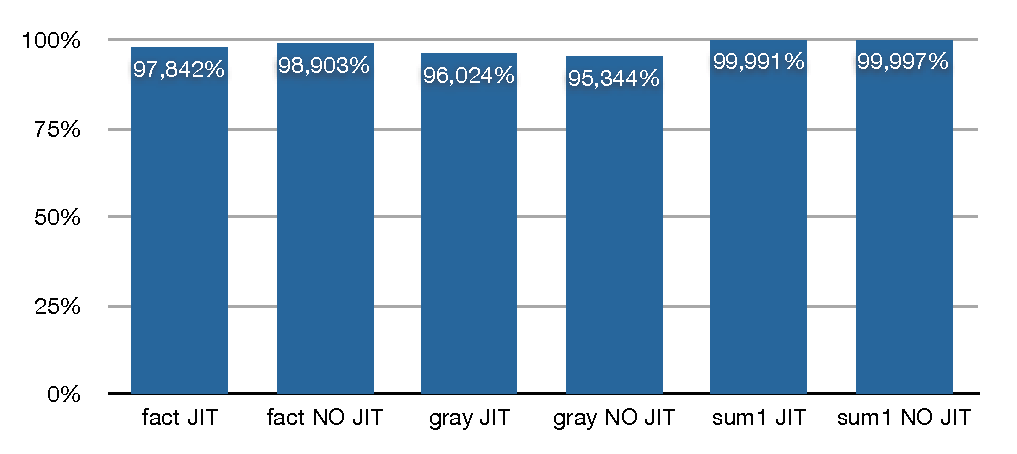
\includegraphics[scale=0.70]{figs/cachel1}
  \caption{Taxa de acerto ao cache L1 \label{fig:cachel1}}
\end{figure}
\begin{figure}[ht!]
  \centering
  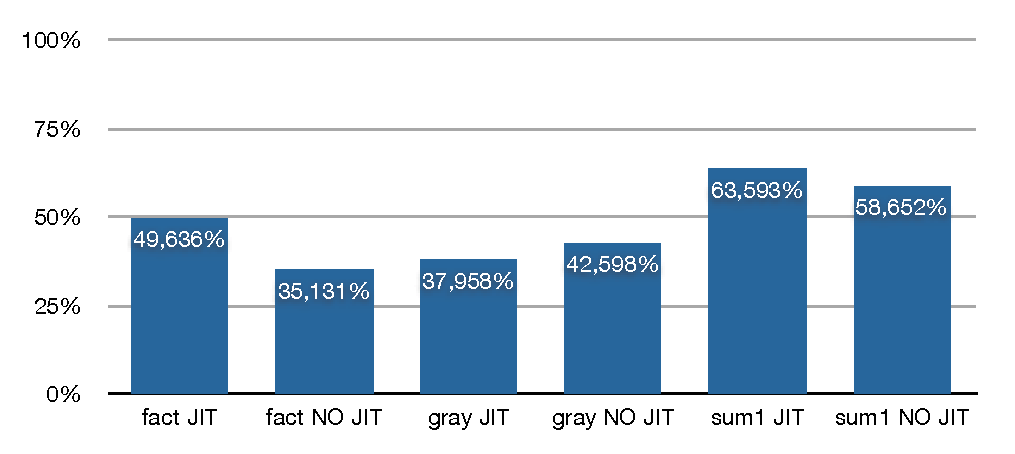
\includegraphics[scale=0.70]{figs/cachel2}
  \caption{Taxa de acerto ao cache L2 \label{fig:cachel2}}
\end{figure}

Somente o \textit{benchmark} \textbf{gray} demonstra uma pequena
vantagem na taxa de acerto ao cache L1, sendo que no geral essa taxa
foi penalizada com o uso do compilador dinâmico. Para o cache L2 a
situação é inversa, apenas o \textbf{gray} teve esta taxa de acerto
reduzida enquanto o \textbf{fact} e \textbf{sum$_1$} aumentaram a
mesma em cerca de 14\% e 5\%, respectivamente. Entretanto, por meio
das duas últimas colunas da Tabela \ref{detalhes2}, verifica-se que o
acesso ao cache L2 foi baixo no geral e, assim, essa taxa de acerto
maior pouco influência no custo de execução.
%De forma geral, o código gerado pelo compilador dinâmico diminuiu a
%taxa de acerto ao cache L1 e aumentou no cache L2. Considerando que o
%código JIT requer uma quantidade significantimente menor de ciclos
%(coluna TOT\_CYC, Tabela \ref{detalhes2}), ... % e que a soma das diferenças
%de falhas entre as colunas \verb!JIT! e \verb!NO JIT! equivale a 

Em relação a desvios incondicionais (Figura \ref{fig:branch}), apenas o
código gerado para o
\textit{benchmark} \textbf{sum$_1$} apresentou melhorias em comparação ao
interpretador. Nos demais casos, houve uma taxa maior de predições
errôneas ao utilizar o código emitido pelo compilador dinâmico. Este
resultado negativo pode estar ligado ao fato dos outros testes terem
um número de $BR\_PRC + BR\_MSP$ baixo quando comparado ao do
\textbf{sum$_1$}, talvez afetando preditores de desvio existentes no
processador utilizado. De qualquer modo, as execuções sem uso do JIT
podem estar indicando um possível ponto de melhoria no interpretador
da linguagem \texttt{Tcl}: forma de \textit{dispatch} de instruções da
máquina virtual. Na implementação atual da \texttt{Tcl}, é feito uso
do método do ``\verb!switch! gigante'' \cite{vmdispatch} que envolve
desvios e custa cerca
de três vezes mais que a técnica \textit{direct threading}
\cite{vmdispatch}.

\begin{figure}[ht!]
  \centering
  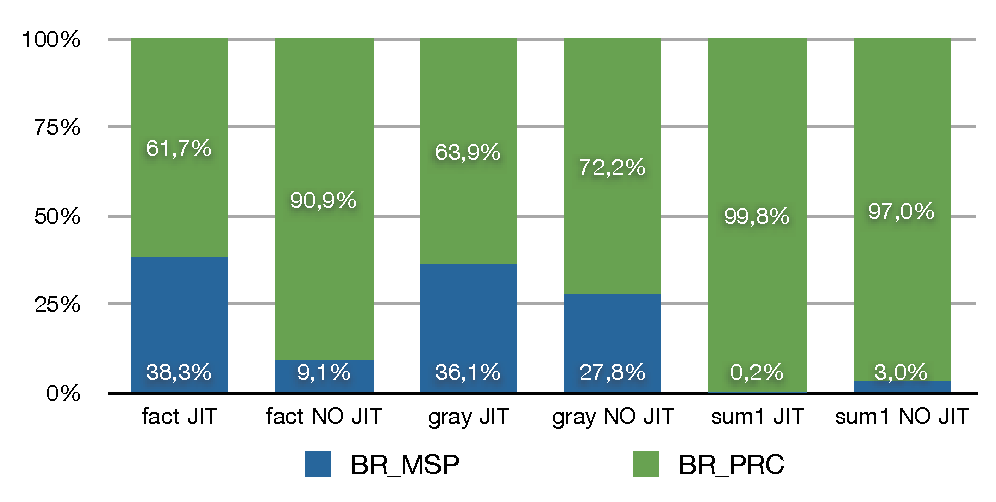
\includegraphics[scale=0.70]{figs/branching}
  \caption{Predição em desvios condicionais \label{fig:branch}}
\end{figure}

Os dados obtidos para o evento RES\_STL (Figura \ref{fig:stalled})
continuam demonstrando que o código
emitido pelo compilador dinâmico é, em geral, pior que aquele emitido pelo gcc.
Proporcionalmente, perde-se mais ciclos por conflito de recursos com o
código do compilador JIT. No pior caso, 66\% dos ciclos do
\textbf{sum$_1$} foram ``desperdiçados'' com JIT ao passo em que
registrou-se apenas 8\% para o mesmo evento na situação sem o JIT.

\begin{figure}[ht!]
  \centering
  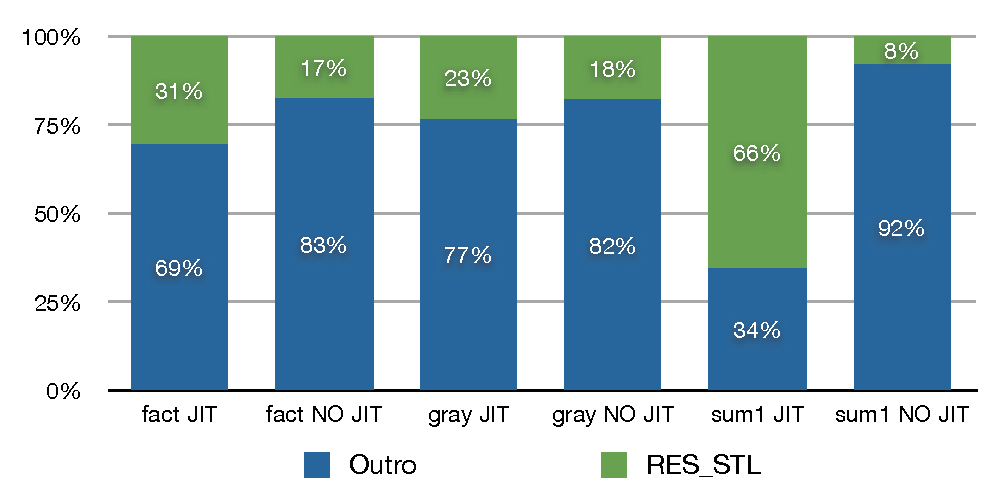
\includegraphics[scale=0.70]{figs/cyclestall}
  \caption{Taxa de ciclos suspensos (\%) \label{fig:stalled}}
\end{figure}

No geral, verificou-se que o código do compilador dinâmico foi
inferior. Isso era esperado por não se tratar de um compilador otimizador.
Assim, a vantagem do compilador JIT são as simplificações realizadas
durante a emissão de código. A Figura \ref{fig:instrelative} apresenta
a quantidade de instruções executadas para o código do compilador JIT
em relação àquela do interpretador.

\begin{figure}[ht!]
  \centering
  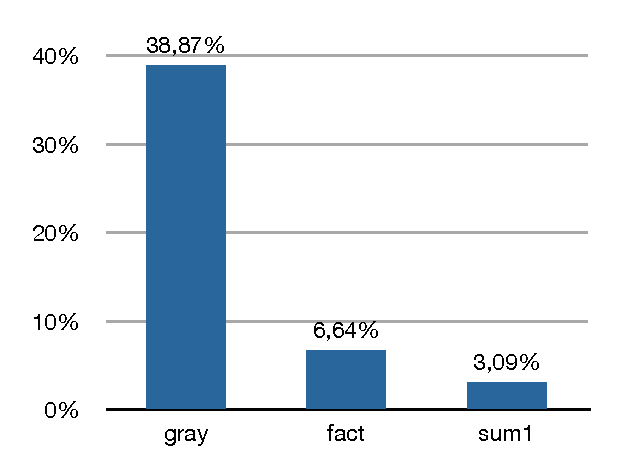
\includegraphics[scale=0.70]{figs/instrelative}
  \caption{Quantidade de instruções executadas em relação ao
    interpretador (\%) \label{fig:instrelative}}
\end{figure}

Com a Figura \ref{fig:instrelative} fica confirmado que,
levando em consideração as análises
anteriores, a redução do
tempo de execução, no caso deste compilador JIT não-otimizador, está
diretamente ligada a
diminuição de instruções necessárias para executar um mesmo
código.
